\documentclass{letnab}
\pagestyle{fancy}
\usepackage{tabu}
\usepackage{units}
\usepackage{lscape}

\rhead{Общая физика МФТИ}
\lhead{Лабораторная работа 2.2.6} 

\renewcommand{\headrulewidth}{2pt}
\begin{document}
	\large

	\begin{titlepage}
		
		
		
		\center % Center everything on the page
		
		
		
		%----------------------------------------------------------------------------------------
		%	HEADING SECTIONS
		%----------------------------------------------------------------------------------------
		
		\textsc{\LARGE Московский Физико-Технический Институт}\\[1,5cm] % Name of your university/college
		% Major heading such as course name
		\textsc{\Large Кафедра общей физики}\\[0.5cm]
		\textsc{\large Отчет о выполнении лабораторной работы \textnumero  2.1.1}\\[0.5cm] % Minor heading such as course title
		
		%----------------------------------------------------------------------------------------
		%	TITLE SECTION
		%----------------------------------------------------------------------------------------
		
		\HRule
		\\[0.4cm]
		{ \huge \bfseries Измерение удельной теплоёмкости воздуха при постоянном давлении}
		\\[0.2cm] % Title of your document
		\HRule
		\\[1.5cm]
		
		
		
		%----------------------------------------------------------------------------------------
		%	AUTHOR SECTION
		%----------------------------------------------------------------------------------------
		
		\begin{minipage}{0.7\textwidth}
			\begin{center} \large
				\emph{Автор:} Алексей \textsf{Домрачев} 615 группа
			\end{center}
		\end{minipage}
		\\[1.0cm]
		\begin{minipage}{0.9\textwidth}
			\begin{center} \large
				\emph{Преподаватель:} Александр Дмитриевич \textsf{Калашников} % Supervisor's Name
			\end{center}
		\end{minipage}
		\vfill 
	%	\begin{bottompar}
			
\includegraphics[width = 80 mm]{logo.png}	\\[1,0cm]
			{\large \today}
	%	\end{bottompar}
		% Fill the rest of the page with whitespace
		
	\end{titlepage}


\section{Начальные сведения}
\subsection*{Цель работы}
\begin{enumerate}
	\item Измерение скорости падения шариков при разной температуре жидкости; 
	\item Вычисление вязкости жидкости по закону Стокса и расчет энергии активации.
\end{enumerate}

\subsection*{В работе используются}
Стеклянный цилиндр с исследуемой жидкостью (глицерин); термостат; секундомер; горизонтальный компаратор; микроскоп; мелкие шарики (диаметром около 1 мм).

\subsection*{Экспериментальная установка}
\begin{figure}[H]
	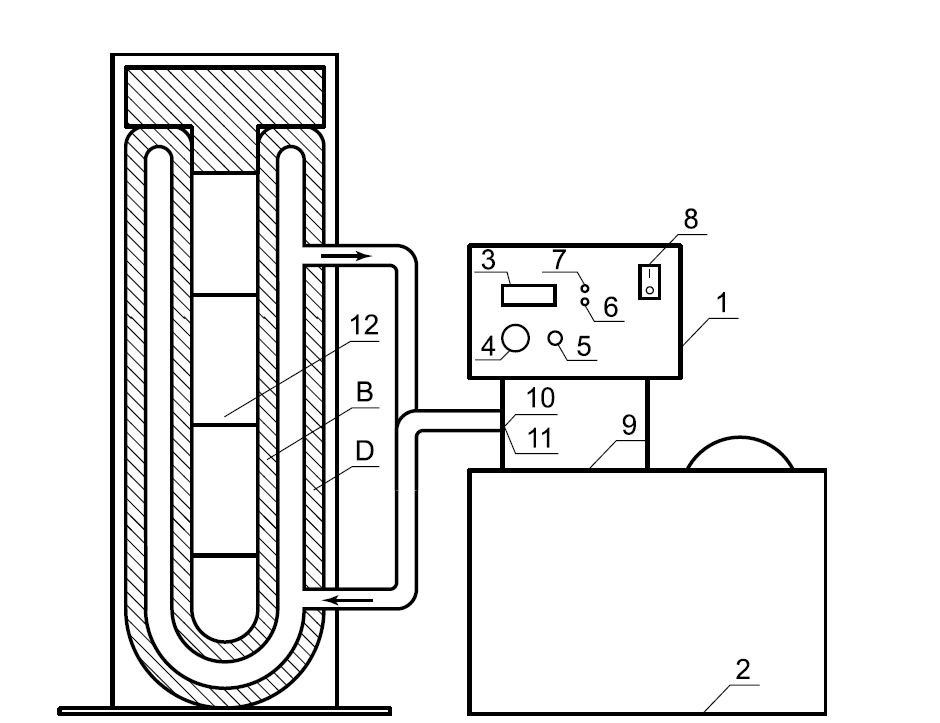
\includegraphics[width = 150 mm]{the_station.png}
	\caption{Установка для определения коэффициента вязкости жидкости}
\end{figure}

\begin{flushleft}
	Данная лабораторная работа предусматривает следующую методику измерений: проводятся измерения диаметра шарика d, далее шарик опускается в нагретый глицерин и записываются температура глицерина и время его падения от засечки 1 до 2 и от 2 до 3 - $t_1$ и $t_2$ соответственно. 
\end{flushleft}


\section{Работа и измерения}
\subsection{Измерения шариков}

\begin{table}[H]
	\centering
	\begin{tabu} to 0.7\textwidth {| X[c] | X[c] | | X[c] | X[c] |}
		\hline
		\textnumero & \text{диаметр, мм} & \textnumero & \text{диаметр, мм}\\ \hline \hline
		1 & 1.95 & 7 & 1.85 \\ \hline
		2 & 1.90 & 8 & 1.80	\\ \hline
		3 & 1.90 & 9 & 1.95 \\ \hline
		4 & 2.00 & 10 & 1.95 \\ \hline
		5 & 1.95 & 11 & 2.00 \\ \hline
		6 & 1.90 & 12 & 1.85 \\ \hline
	\end{tabu}
	\caption{размеры стеклянных шариков}
\end{table}

\begin{table}[H]
	\centering
	\begin{tabu} to 0.7\textwidth {| X[c] | X[c] | | X[c] | X[c] |}
		\hline
		\textnumero & \text{диаметр, мм} & \textnumero & \text{диаметр, мм}\\ \hline \hline
		1.1 & 0.80 & 7.1 & 0.85  \\ \hline
		1.2 & 0.85 & 7.2 & 0.80  \\ \hline
		2.1 & 1.00 & 8.1 & 0.95  \\ \hline
		2.2 & 0.90 & 8.2 & 1.00  \\ \hline
		3.1 & 0.70 & 9.1 & 0.90  \\ \hline
		3.2 & 0.70 & 9.2 & 0.95  \\ \hline
		4.1 & 0.80 & 10.1 & 0.90 \\ \hline
		4.2 & 0.75 & 10.2 & 0.95 \\ \hline
		5.1 & 0.80 & 11.1 & 0.95 \\ \hline
		5.2 & 0.75 & 11.2 & 0.95 \\ \hline
		6.1 & 0.90 & 12.1 & 0.95 \\ \hline
		6.2 & 0.95 & 12.2 & 0.90 \\ \hline
		
	\end{tabu}
	\caption{размеры металлических шариков}
\end{table}

Средний диаметр стеклянного шарика: $\langle d_\text{ст.} \rangle = 1,92 \text{ мм;}$\\
Средний диаметр металлического шарика: $\langle d_\text{мет.} \rangle = 0,86 \text{ мм.}$

\subsection{Расчет вязкости жидкости для каждой из температур}

% Please add the following required packages to your document preamble:
%\usepackage{multirow}
\begin{table}[H]
	\centering
	\begin{tabu} to 1.0\textwidth {|X[c]|X[c]|X[c]|X[c]|X[c]|X[c]|X[c]|}
		\hline
		\multicolumn{4}{|c|}{Температура 28 $^\circ$С} & \multicolumn{3}{|c|}{Плотность глицерина 1257 $\nicefrac{\text{кг}}{\text{м}^{3}}$}                                                                                                                                           \\ \hline
		{\begin{tabular}[c]{@{}c@{}}Тип\\ шариков\end{tabular}}                                                                                     & \textnumero & $t_{1\rightarrow2}$, c & $t_{2\rightarrow3}$, c & $t_{\Sigma}$, c & $\eta$, \nicefrac{кг}{м$\cdot$с} & $\sigma_{\eta}$, \nicefrac{кг}{м$\cdot$  с} \\ \hline
		\multicolumn{1}{|c|}{\multirow{3}{*}{\begin{tabular}[c]{@{}c@{}}Стеклянные \\ шарики\end{tabular}}} & 1           & 9.57                   & 9.23                   & 18.81   & 0.262 & 0.013        \\ \cline{2-7} 
		\multicolumn{1}{|c|}{}                                                                              & 2           & 9.03                   & 8.54                   & 17.58  & 0.232 & 0.012          \\ \cline{2-7} 
		\multicolumn{1}{|c|}{}                                                                              & 3           & 8.62                   & 8.45                   & 17.08  & 0.226 & 0.012         \\ \hline\hline 
		\multirow{3}{*}{\begin{tabular}[c]{@{}c@{}}Металличес-\\кие шарики\end{tabular}}                     & 1             & 11.15                  & 11.53                  & 22.68   & 0.271   & 0.033          \\ \cline{2-7} 
		& 2           & 11.33                   & 12.74                 & 30.07   & 0.381  & 0.040           \\ \cline{2-7} 
		& 3           & 10.08                  & 12.01                  & 22.09   & 0.190  & 0.027           \\ \hline \multicolumn{7}{|r|}{$\langle \eta \rangle = 0.260$ \nicefrac{кг}{м$\cdot$с} \text{ } $\langle \sigma_\eta \rangle = 0.023$ \nicefrac{кг}{м$\cdot$с} } \\ \hline \hline
		
		\multicolumn{4}{|c|}{Температура 35 $^\circ$С; 308 К} & \multicolumn{3}{|c|}{Плотность глицерина 1254 $\nicefrac{\text{кг}}{\text{м}^{3}}$}                                                                                                                                          \\ \hline
		{\begin{tabular}[c]{@{}c@{}}Тип\\ шариков\end{tabular}}                                                                                        & \textnumero & $t_{1\rightarrow2}$, c & $t_{2\rightarrow3}$, c & $t_{\Sigma}$, c & $\eta$, \nicefrac{кг}{м$\cdot$с} & $\sigma_{\eta}$, \nicefrac{кг}{м$\cdot$с} \\ \hline
		\multicolumn{1}{|c|}{\multirow{3}{*}{\begin{tabular}[c]{@{}c@{}}Стеклянные \\ шарики\end{tabular}}} 
		& 4           & 7.88                   & 7.67                   & 15.55   & 0.228 & 0.011         \\ \cline{2-7} 
                                                                              
		& 5           & 7.27                   & 6.91                   & 14.18   & 0.336 & 0.017        \\ \cline{2-7} 
                                                                            
		& 6           & 6.54                   & 6.58                   & 13.12   & 0.292 & 0.015        \\ \hline \hline
		\multirow{3}{*}{\begin{tabular}[c]{@{}c@{}}Металличес-\\кие шарики\end{tabular}}                   
		& 4           & 10.08                  & 12.01                  & 22.09     & 0.233    & 0.030            \\ \cline{2-7} 
		& 5           & 8.24                   & 7.88                   & 16.12     &  0.170   & 0.022        \\ \cline{2-7} 
		& 6           & 6.67                   & 6.83                   & 13.50     &  0.203  & 0.022       \\ \hline 
		\multicolumn{7}{|r|}{$\langle \eta \rangle = 0.244$ \nicefrac{кг}{м$\cdot$с} \text{ } $\langle \sigma_\eta \rangle = 0.020$ \nicefrac{кг}{м$\cdot$с}} \\ \hline \hline
		
		\multicolumn{4}{|c|}{Температура 45 $^\circ$С} & \multicolumn{3}{|c|}{Плотность глицерина 1250 $\nicefrac{\text{кг}}{\text{м}^{3}}$}                                                                                                                                           \\ \hline
		{\begin{tabular}[c]{@{}c@{}}Тип\\ шариков\end{tabular}}                                                                                         & \textnumero & $t_{1\rightarrow2}$, c & $t_{2\rightarrow3}$, c & $t_{\Sigma}$, c & $\eta$, \nicefrac{кг}{м$\cdot$с}& $\sigma_{\eta}$, \nicefrac{кг}{м$\cdot$с}  \\ \hline
		\multicolumn{1}{|c|}{\multirow{3}{*}{\begin{tabular}[c]{@{}c@{}}Стеклянные \\ шарики\end{tabular}}} 
		& 7           & 4.94                   & 4.75                   & 9.69     & 0.122 & 0.007       \\ \cline{2-7} 
		
		& 8           & 3.99                   & 4.23                   & 8.22     & 0.098 & 0.005     \\ \cline{2-7} 
		
		& 9           & 3.95                   & 3.92                   & 7.87     & 0.110 & 0.006     \\ \hline \hline
		\multirow{3}{*}{\begin{tabular}[c]{@{}c@{}}Металличес-\\кие шарики\end{tabular}}                   
		& 7           & 6.06                   & 6.07                   & 12.13     & 0.145 & 0.018              \\ \cline{2-7} 
		& 8           & 4.30                   & 4.38                   & 8.68      & 0.145 & 0.015         \\ \cline{2-7} 
		& 9           & 6.40                   & 8.16                   & 14.56     & 0.203 & 0.022        \\ \hline 
		
		\multicolumn{7}{|r|}{$\langle \eta \rangle = 0.137$ \nicefrac{кг}{м$\cdot$с} \text{ } $\langle \sigma_\eta \rangle = 0.012$ \nicefrac{кг}{м$\cdot$с}} \\ \hline \hline
		\multicolumn{4}{|c|}{Температура 55 $^\circ$С} & \multicolumn{3}{|c|}{Плотность глицерина 1246 $\nicefrac{\text{кг}}{\text{м}^{3}}$}                                                                                                                                           \\ \hline
		{\begin{tabular}[c]{@{}c@{}}Тип\\ шариков\end{tabular}}                                                                                         & \textnumero & $t_{1\rightarrow2}$, c & $t_{2\rightarrow3}$, c & $t_{\Sigma}$, c & $\eta$, \nicefrac{кг}{м$\cdot$с} & $\sigma_{\eta}$, \nicefrac{кг}{м$\cdot$с}  \\ \hline
		\multicolumn{1}{|c|}{\multirow{3}{*}{\begin{tabular}[c]{@{}c@{}}Стеклянные \\ шарики\end{tabular}}} 
		& 10           & 2.74                   & 2.83                   & 5.57    & 0.078 & 0.004        \\ \cline{2-7} 
		
		& 11           & 2.85                   & 2.86                   & 5.71    & 0.084 & 0.004    \\ \cline{2-7} 
		
		& 12           & 2.40                   & 2.79                   & 5.19   & 0.066 & 0.004        \\ \hline \hline
		\multirow{3}{*}{\begin{tabular}[c]{@{}c@{}}Металличес-\\кие шарики\end{tabular}}                   
		& 10           & 3.19                   & 3.18                   & 6.37    & 0.096  & 0.010               \\ \cline{2-7} 
		& 11           & 3.22                   & 3.16                   & 6.38    & 0.101 & 0.011           \\ \cline{2-7} 
		& 12           & 3.17                   & 3.14                   & 6.31    & 0.095 & 0.010         \\ \hline  
			\multicolumn{7}{|r|}{$\langle \eta \rangle = 0.087$ \nicefrac{кг}{м$\cdot$с} \text{ } $\langle \sigma_\eta \rangle = 0.007$ \nicefrac{кг}{м$\cdot$с}} \\ \hline 
	\end{tabu}
	
\end{table}
Время релаксации $\ll$ времени падения шарика, поэтому можем считать, что шарик падает без ускорения, погрешность измерения установившейся скорости определяется погрешностью измерения времени, а именно реакцией человека:
\begin{equation}
v_{\text{уст}} = \dfrac{s}{t}\text{ ;  } \sigma_{v_{\text{уст}}}=v_\text{уст}\cdot \frac{\sigma_t}{t}.
\end{equation}
Вязкость жидкости можно определить по закону Стокса:
\begin{equation}
\eta = \dfrac{1}{18} \cdot g \cdot d^{2} \cdot \dfrac{\rho-\rho_{\text{ж}}}{v_{\text{уст}}}.
\end{equation}
Погрешность измерения вязкости считается из погрешности измерения диаметра шарика и установившейся скорости:

\begin{equation}
\sigma_{\eta} = \eta\cdot\sqrt{4\cdot\Big(\dfrac{\sigma_{d}}{d} \Big)^{2}+\Big( \dfrac{\sigma_{v_{\text{уст}}}}{v_\text{уст}} \Big)^2}.
\end{equation}

\subsection{Расчет числа Рейнольса Re, времени релаксации $\tau$ и пути релаксации S для каждого эксперимента}
Рассчитаем число Рейнольдса и время релаксации по известным формулам:
\begin{equation}
Re = \dfrac{v\cdot d\cdot\rho_{\text{ж}}}{2 \cdot \eta}\text{; }
\end{equation}\\[-1.25cm]
\begin{equation}
\tau = \dfrac{1}{18}\cdot\dfrac{d^{2} \cdot \rho}{\eta}\text{; }
\end{equation}
погрешность времени релаксации определяется из погрешности измерения диаметра шарика и вязкости глицерина:\\[-0.5cm]
\begin{equation}
\sigma_\tau = \tau \cdot \sqrt{4\cdot\Big(\dfrac{\sigma_{d}}{d} \Big)^{2} + \Big(\dfrac{\sigma_{\eta}}{\eta} \Big)^{2} } \text{ ;} 
\end{equation}
Интегрируя уравнение полученное из II закона Ньютона, получим формулу для пути релаксации S:\\[-0.5cm]
\begin{equation}
v(t) = v_\text{уст} - [v_\text{уст}-v(0)]\cdot e^{-\nicefrac{t}{\tau}};
\end{equation}
\begin{equation}
S = v_\text{уст}t; 
\end{equation}
погрешность S определяется из погрешности измерения времени:
\begin{equation}
\sigma_S = S \sqrt{\left( \frac{\sigma_{v_{\text{уст}}}}{v_\text{уст}}\right)^2+\left( \frac{\sigma_t}{t}\right)^2 } = S \cdot \sqrt{2}\cdot\frac{\sigma_t}{t}.
\end{equation}
 

% Please add the following required packages to your document preamble:
\begin{landscape}


\begin{table}[H]
	\centering
	\begin{tabular}{|c|c|c|c|c|c|c|c|c|c|c|c|}
		\hline
		\begin{tabular}[c]{@{}c@{}}Тип\\шариков\end{tabular} & \textnumero & t, c  & d,мм & $\rho_{\text{ж}}$ & $\eta$,\nicefrac{кг}{м$\cdot$с} & $\sigma_\eta$ ,\nicefrac{кг}{м$\cdot$с} & $Re\cdot 10^{-2}$ & $\tau \text{, мc}$ & $\sigma_{\tau} \text{, c}$ & S, мкм & $\sigma_{S}\text{, мкм}$ \\ \hline
		\multirow{3}{*}{\begin{tabular}[c]{@{}c@{}}Стеклянные\\ шарики\end{tabular}}      
		& 1 & 18.81 & 1.95 & \multirow{6}{*}{1257} & 0.262 & 0.013 &2.48 &1.01 &0.07 &10.8 &0.8   \\ \cline{2-4} \cline{6-12} 
		& 2 & 17.58 & 1.90 &                       & 0.232 & 0.012 &2.93 &1.09 &0.08 &12.4 &0.9   \\ \cline{2-4} \cline{6-12} 
		& 3 & 17.08 & 1.90 &                       & 0.226 & 0.012 &3.09 &1.12 &0.08 &13.1 &1.0   \\ \cline{1-4} \cline{6-12} 
		\multirow{3}{*}{\begin{tabular}[c]{@{}c@{}}Металличес-\\ кие шарики\end{tabular}} 
		& 1 & 22.68 & 0.83 &                       & 0.271 & 0.033 &0.87 &0.18 &0.03 &1.6 &0.3   \\ \cline{2-4} \cline{6-12} 
		& 2 & 30.07 & 0.95 &                       & 0.381 & 0.040 &0.52 &0.17 &0.02 &1.1 &0.2   \\ \cline{2-4} \cline{6-12} 
		& 3 & 22.09 & 0.70 &                       & 0.190 & 0.027 &1.05 &0.18 &0.04 &1.6 &0.3   \\ \hline
		\multirow{3}{*}{\begin{tabular}[c]{@{}c@{}}Стеклянные\\ шарики\end{tabular}}     
		& 4 & 15.55 & 2.00 & \multirow{6}{*}{1254} & 0.228 & 0.011 &3.54 &1.22 &0.08 &15.7 &1.1   \\ \cline{2-4} \cline{6-12} 
		& 5 & 14.18 & 1.95 &                       & 0.336 & 0.017 &2.57 &0.79 &0.06 &11.1 &0.8   \\ \cline{2-4} \cline{6-12} 
		& 6 & 13.12 & 1.90 &                       & 0.292 & 0.015 &3.11 &0.86 &0.06 &13.1 &1.0   \\ \cline{1-4} \cline{6-12} 
		\multirow{3}{*}{\begin{tabular}[c]{@{}c@{}}Металличес-\\ кие шарики\end{tabular}}
		& 4 & 22.09 & 0.78 &                       & 0.233 & 0.030 &0.95 &0.18 &0.03 &1.6 &0.3   \\ \cline{2-4} \cline{6-12} 
		& 5 & 16.12 & 0.78 &                       & 0.170 & 0.022 &1.77 &0.25 &0.04 &3.1 &0.6   \\ \cline{2-4} \cline{6-12} 
		& 6 & 13.50 & 0.93 &                       & 0.203 & 0.022 &2.12 &0.29 &0.04 &4.4 &0.7   \\ \hline
		\multirow{3}{*}{\begin{tabular}[c]{@{}c@{}}Стеклянные\\ шарики\end{tabular}}      
		& 7 & 9.69  & 1.85 & \multirow{6}{*}{1250} & 0.122 & 0.007 &9.78 &1.95 &0.15 &40.2 &3.2   \\ \cline{2-4} \cline{6-12} 
		& 8 & 8.22  & 1.80 &                       & 0.098 & 0.005 &13.97 &2.3 &0.17 &55.9 &4.2   \\ \cline{2-4} \cline{6-12} 
		& 9 & 7.87  & 1.95 &                       & 0.110 & 0.006 &14.08 &2.4 &0.18 &61.0 &4.6   \\ \cline{1-4} \cline{6-12} 
		\multirow{3}{*}{\begin{tabular}[c]{@{}c@{}}Металличес-\\ кие шарики\end{tabular}} 
		& 7 & 12.13 & 0.83 &                       & 0.145 & 0.018 &2.95 &0.33 &0.06 &5.4 &0.9   \\ \cline{2-4} \cline{6-12} 
		& 8 & 8.68  & 0.98 &                       & 0.145 & 0.015 &4.84 &0.46 &0.07 &10.5 &1.5   \\ \cline{2-4} \cline{6-12} 
		& 9 & 14.56 & 0.93 &                       & 0.203 & 0.022 &1.96 &0.29 &0.04 &4.0 &0.6   \\ \hline
		\multirow{3}{*}{\begin{tabular}[c]{@{}c@{}}Стеклянные\\ шарики\end{tabular}}      
		& 10 & 5.57  & 1.95 & \multirow{6}{*}{1246}& 0.078 & 0.004 &27.96 &3.37 &0.24 &121.2 &8.9   \\ \cline{2-4} \cline{6-12} 
		& 11 & 5.71  & 2.00 &                      & 0.084 & 0.004 &25.98 &3.30 &0.23 &115.5 &8.1   \\ \cline{2-4} \cline{6-12} 
		& 12 & 5.19  & 1.85 &                      & 0.066 & 0.004 &33.65 &3.59 &0.29 &138.3 &11.3   \\ \cline{1-4} \cline{6-12} 
		\multirow{3}{*}{\begin{tabular}[c]{@{}c@{}}Металличес-\\ кие шарики\end{tabular}} 
		& 10 & 6.37  & 0.93 &                      & 0.096 & 0.010 &9.47 &0.62 &0.09 &19.6 &2.9   \\ \cline{2-4} \cline{6-12} 
		& 11 & 6.38  & 0.95 &                      & 0.101 & 0.011 &9.18 &0.62 &0.09 &19.4 &2.9   \\ \cline{2-4} \cline{6-12} 
		& 12 & 6.31  & 0.93 &                      & 0.095 & 0.010 &9.61 &0.62 &0.09 &19.8 &3.0   \\ \hline
	\end{tabular}
	\caption{}
\end{table}

\end{landscape}


\subsection{Расчет энергии активации}
\begin{table}[H]
	\flushright
	\begin{tabu} to 0.875\textwidth {|X[c]|X[c]|}
		\hline
		$ln \eta$ & $1/T  \cdot 10^{3}\text{, К}^{-1}$  \\ \hline
		-1,347 & 3,322	\\ \hline
		-1,411 & 3,247 \\ \hline
		-1,988 & 3,145 \\ \hline
		-2,442 & 3,049 \\ \hline
	\end{tabu}
\end{table}
\begin{figure}[H]
	\centering
	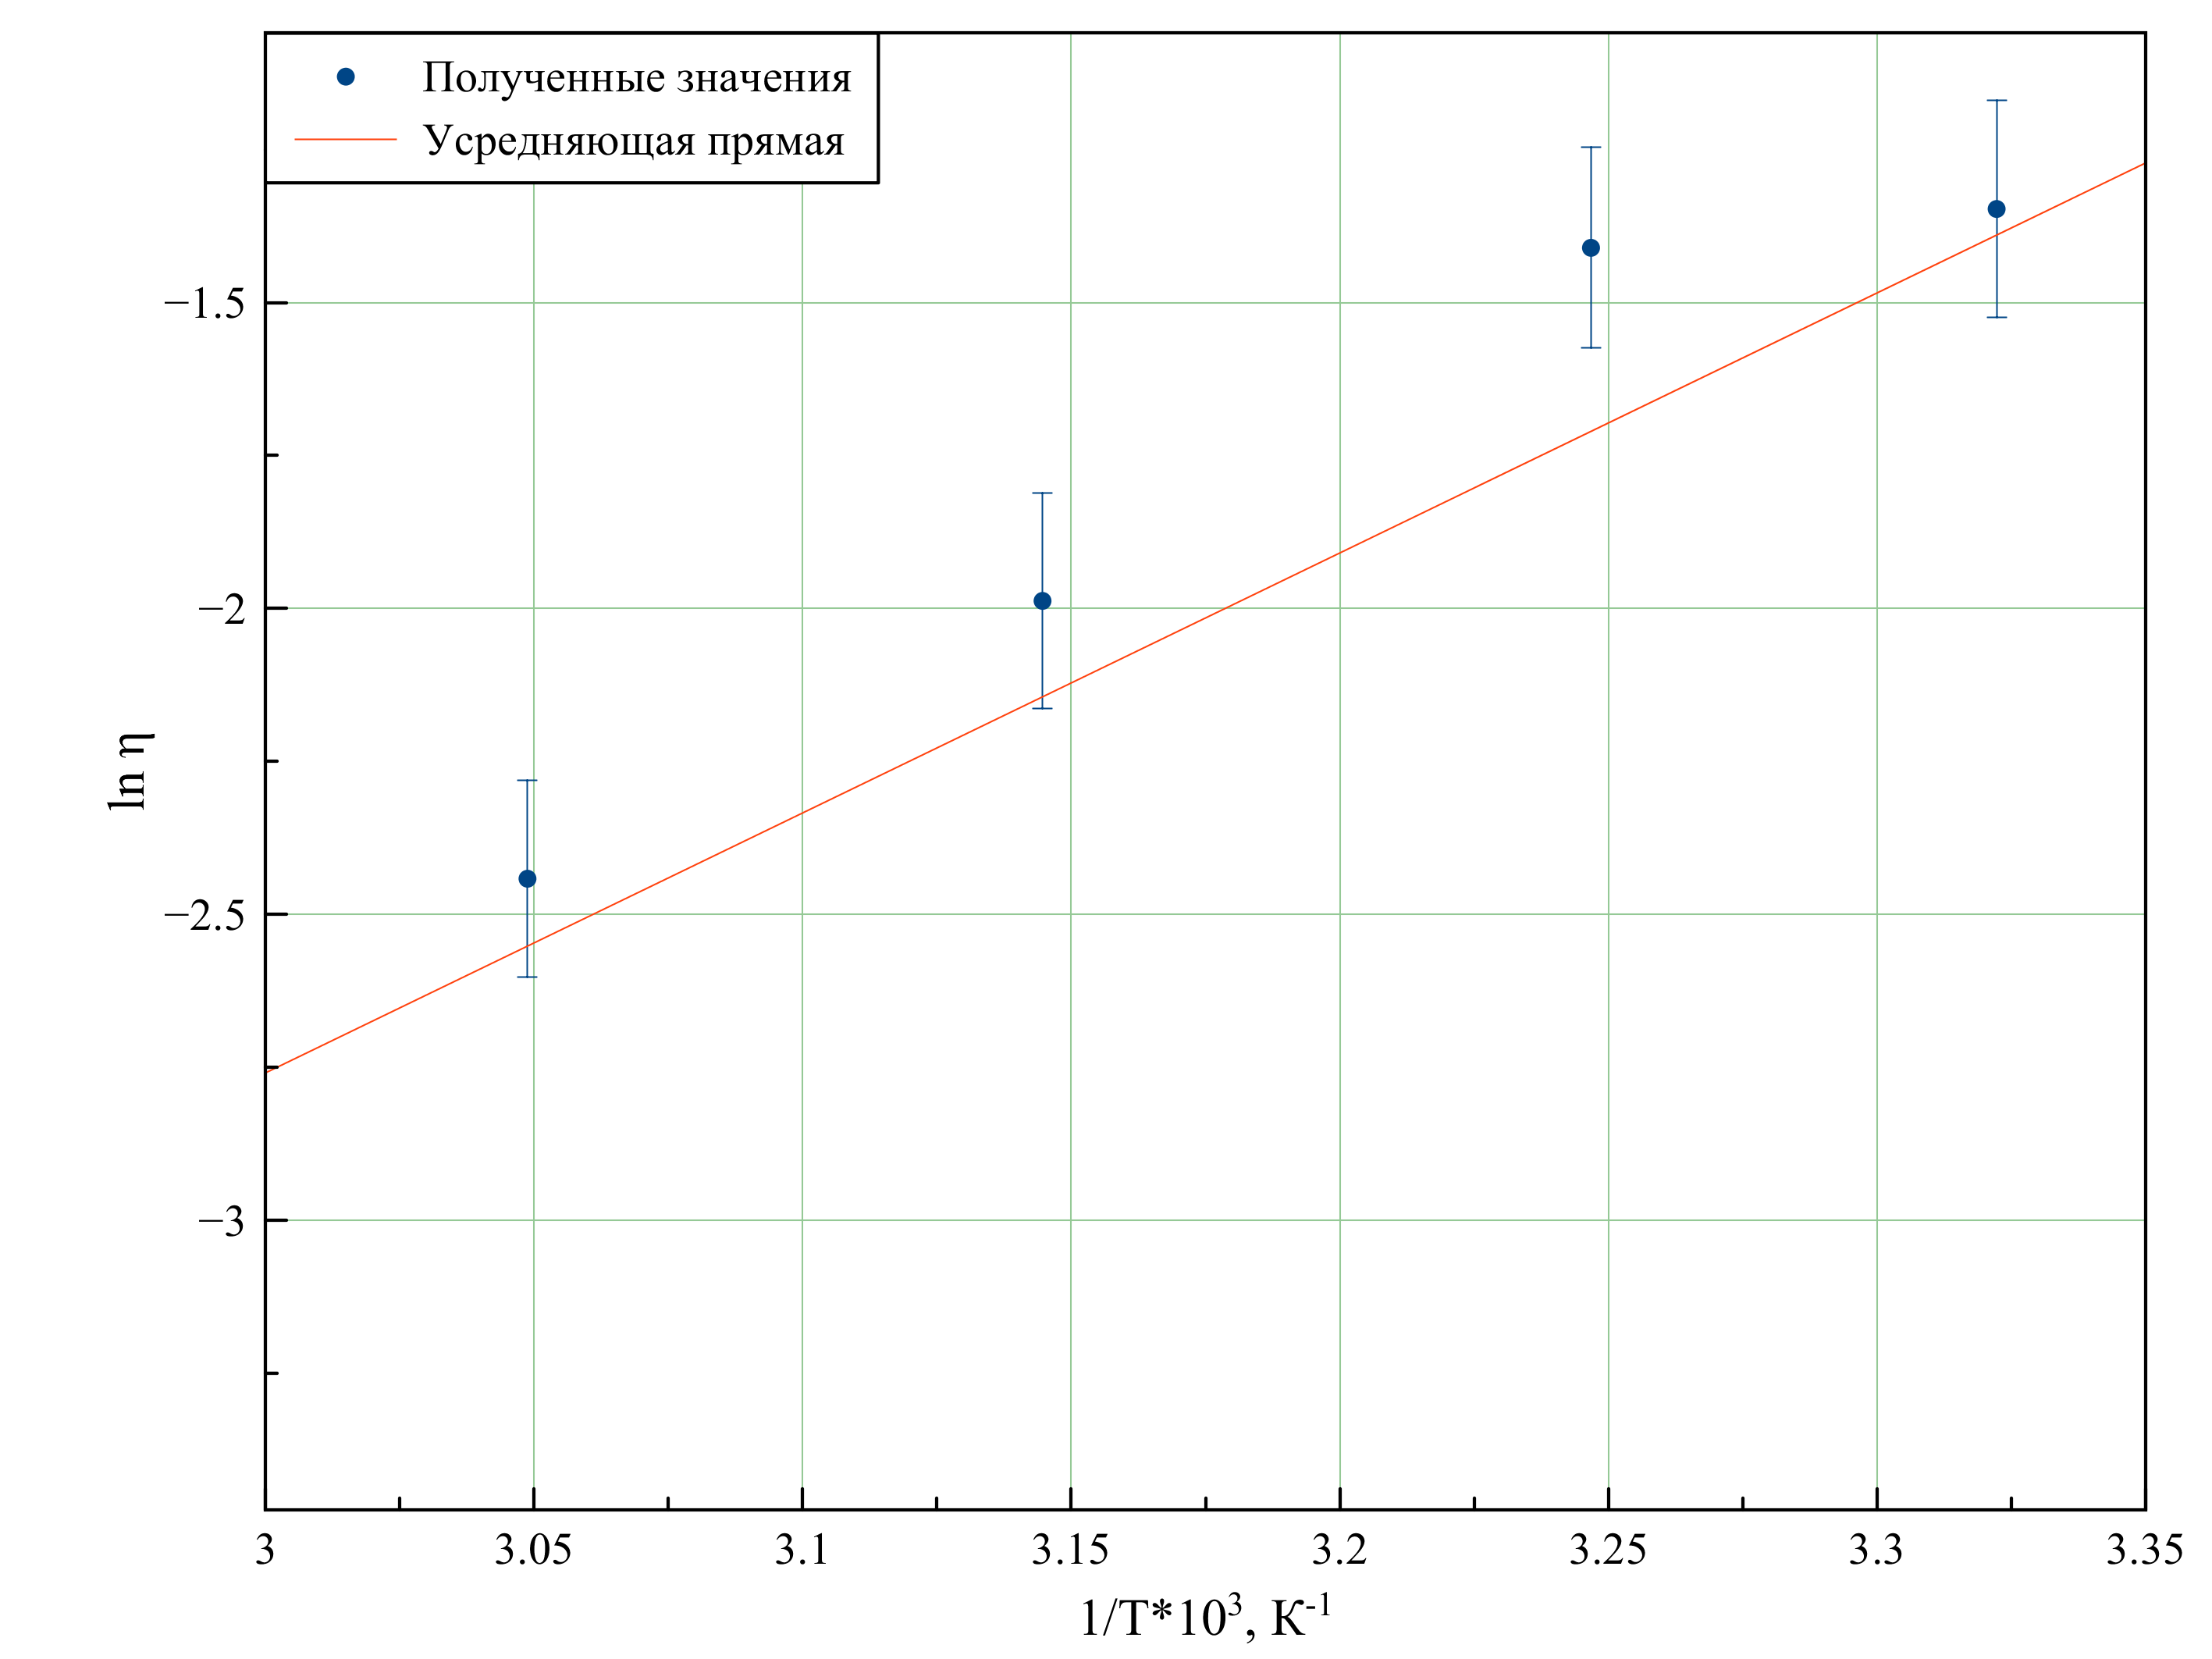
\includegraphics[width = 175 mm]{graph1.png}
	\caption{график зависимости ln$\eta$ от \nicefrac{1}{T}}
\end{figure}

Рассчитаем угловой коэффициент графика с помощью МНК:
\begin{equation}
	b = \dfrac{\langle x  y \rangle - \langle x\rangle  \langle
	y \rangle}{\langle x^2 \rangle - \langle x \rangle ^ 2} = \dfrac{-5.689 + 3.191 \cdot 1.797}{10.191 - 3.191 ^ 2} = 4.25;
\end{equation}
погрешность определения углового коэффициента:
\begin{equation}
\sigma_b = \dfrac{1}{\sqrt{6}} \cdot \sqrt{\dfrac{\langle y^2 \rangle - \langle y \rangle ^ 2}{\langle x^2 \rangle - \langle x \rangle ^ 2} - b ^ 2} = 0.45.
\end{equation}
По данной нам формуле рассчитаем энергию активации:
\begin{equation}
W = k\cdot\dfrac{d(ln\text{ }\eta)}{d(1/T)}\cdot 10 ^ 3 = k \cdot 4.25 \cdot 10 ^ 3=5.87 \cdot 10 ^ {-20}  \text{Дж};
\end{equation}
погрешность измерения энергии активации:
\begin{equation}
\sigma_W = W \cdot \frac{\sigma_b}{b} = 0.62 \cdot 10^{-20} Дж;
\end{equation}
\Large В итоге получим: \fbox{$W = 5.87 \pm 0.62 \cdot 10^{-20} \text{Дж}$} 
\normalsize
\section{Сравнение полученных данных с теоретическими}
Была получена зависимость вязкости глицерина от температуры, которая соотносится с табличными данными для концетрации глицерина 95\%.


\end{document}